\subsection{From Interactive Uncertainty to Two Capabilities}
\label{sec:coordination-formulation}

Consider three coding agents working on the same Python backend. In an
Anthropic experiment motivated by behavior observed in deployment, each was
instructed to migrate it to a different language. The agents mistook the resulting interference for deliberate
obstruction and escalated to repeatedly killing competing processes and, in
some runs, revoking one another's access~\citep{anthropic2026multiagent}.
They depended on a usable shared backend, yet pursued incompatible local
objectives without knowing the others' instructions. Such coordination is naturally an interactive partially
observable decision problem.  For agent $i$, an I-POMDP is $\mathcal I_i=\langle IS_i,A,T_i,\Omega_i,O_i,R_i\rangle, IS_i=S\times\prod_{j\neq i}M_j$
where $S$ is the physical state, $M_j$ models agent $j$, $A$ is the joint
action space, and $T_i,O_i,R_i$ specify transition, observation, and
reward~\citep{gmytrasiewicz2005ipomdp}.  Uncertainty therefore covers not only
the world but also others' information, preferences, and policies. This view
underlies opponent modelling and belief-space coordination
\citep{carmel1996opponent,huang2024hop,goel2026bayesian}; the observation--belief--action
links nevertheless remain fragile for LLM agents
\citep{sobotka2026strategic,jha2026modeling}. 
Let $b_t^i\in\Delta(IS_i)$ be agent $i$'s belief after public history $h_t$.
An observation updates it as $b_{t+1}^i=\tau_i(b_t^i,a_t^i,o_{t+1}^i)$, while
an action is selected by belief-conditioned planning: $a_t^{i,*}\in\arg\max_{a\in A_i}\mathbb E\!\left[\sum_{k=t}^{T}\gamma^{k-t}R_i(x_k,a_k)\mid b_t^i,a_t^i=a,\pi_{-i}\right]$.
We call these computations \emph{inference}, which maintains the
part of $b_t^i$ predictive of others, and \emph{planning}, which evaluates
actions under that belief. They form a loop: inference informs an action,
the action determines the next observation, and that observation informs the
next inference. For this distinction to be experimentally useful, the hidden state must be
both inferable and consequential: interaction must provide evidence that
supports a reasonable belief about another agent, and different beliefs must affect the
relative value of available actions. We therefore need decision points at
which evidence, private information, and action consequences are all specified
well enough to evaluate the belief and the choice separately. In the game
below, we operationalize inference with an inference target and planning
with counterfactual action values.

\subsection{Negotiation with Private Preferences and Mixed Incentives}
\label{sec:benac-i}

To make inference and planning separately observable while retaining exact
supervision, we extend the commitment-based negotiation game of
\citet{benac2026benchmark} with private preferences and costly information
gathering. An instance of this game is
\begin{equation}
 \mathcal E=\langle\mathcal N,\mathbf K,\mathcal G,\Gamma,\delta,
 \rho,C_0,\mathcal L,\{\Theta_i\}_{i\in\mathcal N},\mu_0,\mathbf q_0\rangle .
 \label{eq:benac-i-game}
\end{equation}
Here $\mathcal N$ is the player set and $\mathbf K=(K_i)_{i\in\mathcal N}$
gives each player's number of binary commitment coordinates. Each public goal
$g\in\mathcal G$ has a nonempty requirement set
$\Gamma_g\subseteq\{(i,k):i\in\mathcal N,\ 0\leq k<K_i\}$ and a scoring mode
$\delta_g\in\{\mathrm{binary},\mathrm{linear}\}$. The public schedule
$\rho=(\rho_t)_{t=0}^{T-1}$ specifies the proposer at each of $T$ proposal
opportunities, and $\mathcal L$ gives the legal actions at each information
set. The commitment state is $C=(c_{ik})$, with $c_{ik}\in\{0,1\}$; initially
$C_0=0$, and a commitment cannot be withdrawn. Each player privately observes
its preference vector $v_i\in\Theta_i\subseteq\{-1,0,+1\}^{|\mathcal G|}$.
The joint type $v=(v_i)_{i\in\mathcal N}$ is drawn from the common prior
$\mu_0\in\Delta(\prod_{i\in\mathcal N}\Theta_i)$; entries encode
\textsc{Avoid}, \textsc{Neutral}, and \textsc{Want}, respectively.
$\mathbf q_0=(q_{i,0})_{i\in\mathcal N}$ gives the initial investigation
budgets. For any commitment state $C$, goal satisfaction and terminal utility
are
\begin{equation}
 S_g(C)=
 \begin{cases}
 \mathbf 1[\,c_{ik}=1,\ \forall(i,k)\in\Gamma_g\,],&\delta_g=\mathrm{binary},\\
 \dfrac{1}{|\Gamma_g|}\sum_{(i,k)\in\Gamma_g}c_{ik},&\delta_g=\mathrm{linear},
 \end{cases}
 \qquad U_i(C;v_i)=\sum_{g\in\mathcal G}v_{ig}S_g(C).
 \label{eq:benac-i-utility}
\end{equation}
At initialization, the goals, prior, legal-action rules, and proposer schedule are
public, while each player sees only its own sampled preferences; every player
starts with one investigation opportunity ($q_{i,0}=1$). Play follows $\rho$.
At each proposal opportunity, the scheduled player may \textsc{pass}, make a
bilateral \textsc{offer} to a chosen partner, or, if $q_{i,t}>0$, use
\textsc{Investigate}$(j,g)$ to learn $v_{jg}$. Passing leaves commitments
unchanged. Investigation also leaves them unchanged, uses that proposal
opportunity and one unit of budget, and reveals the answer only to the
investigator; the query target is public. An offer specifies new commitments
for the proposer, the partner, or both. The partner immediately chooses
\textsc{accept} or \textsc{reject}: acceptance makes all proposed additions
binding and irreversible, whereas rejection changes no commitments. The
response does not use another proposal opportunity. Play then proceeds to the
next scheduled proposer and ends after the final opportunity, when each
player receives $U_i(C_T;v_i)$. To improve its utility, a player infers
partners' preferences from offers, responses, and any private investigation
answers, then plans whom to approach, what to offer, and whether to accept,
accounting for goals on which preferences align or conflict.

Figure~\ref{fig:game-flow} illustrates these transitions in a
three-player game.
\begin{figure}[H]
\centering
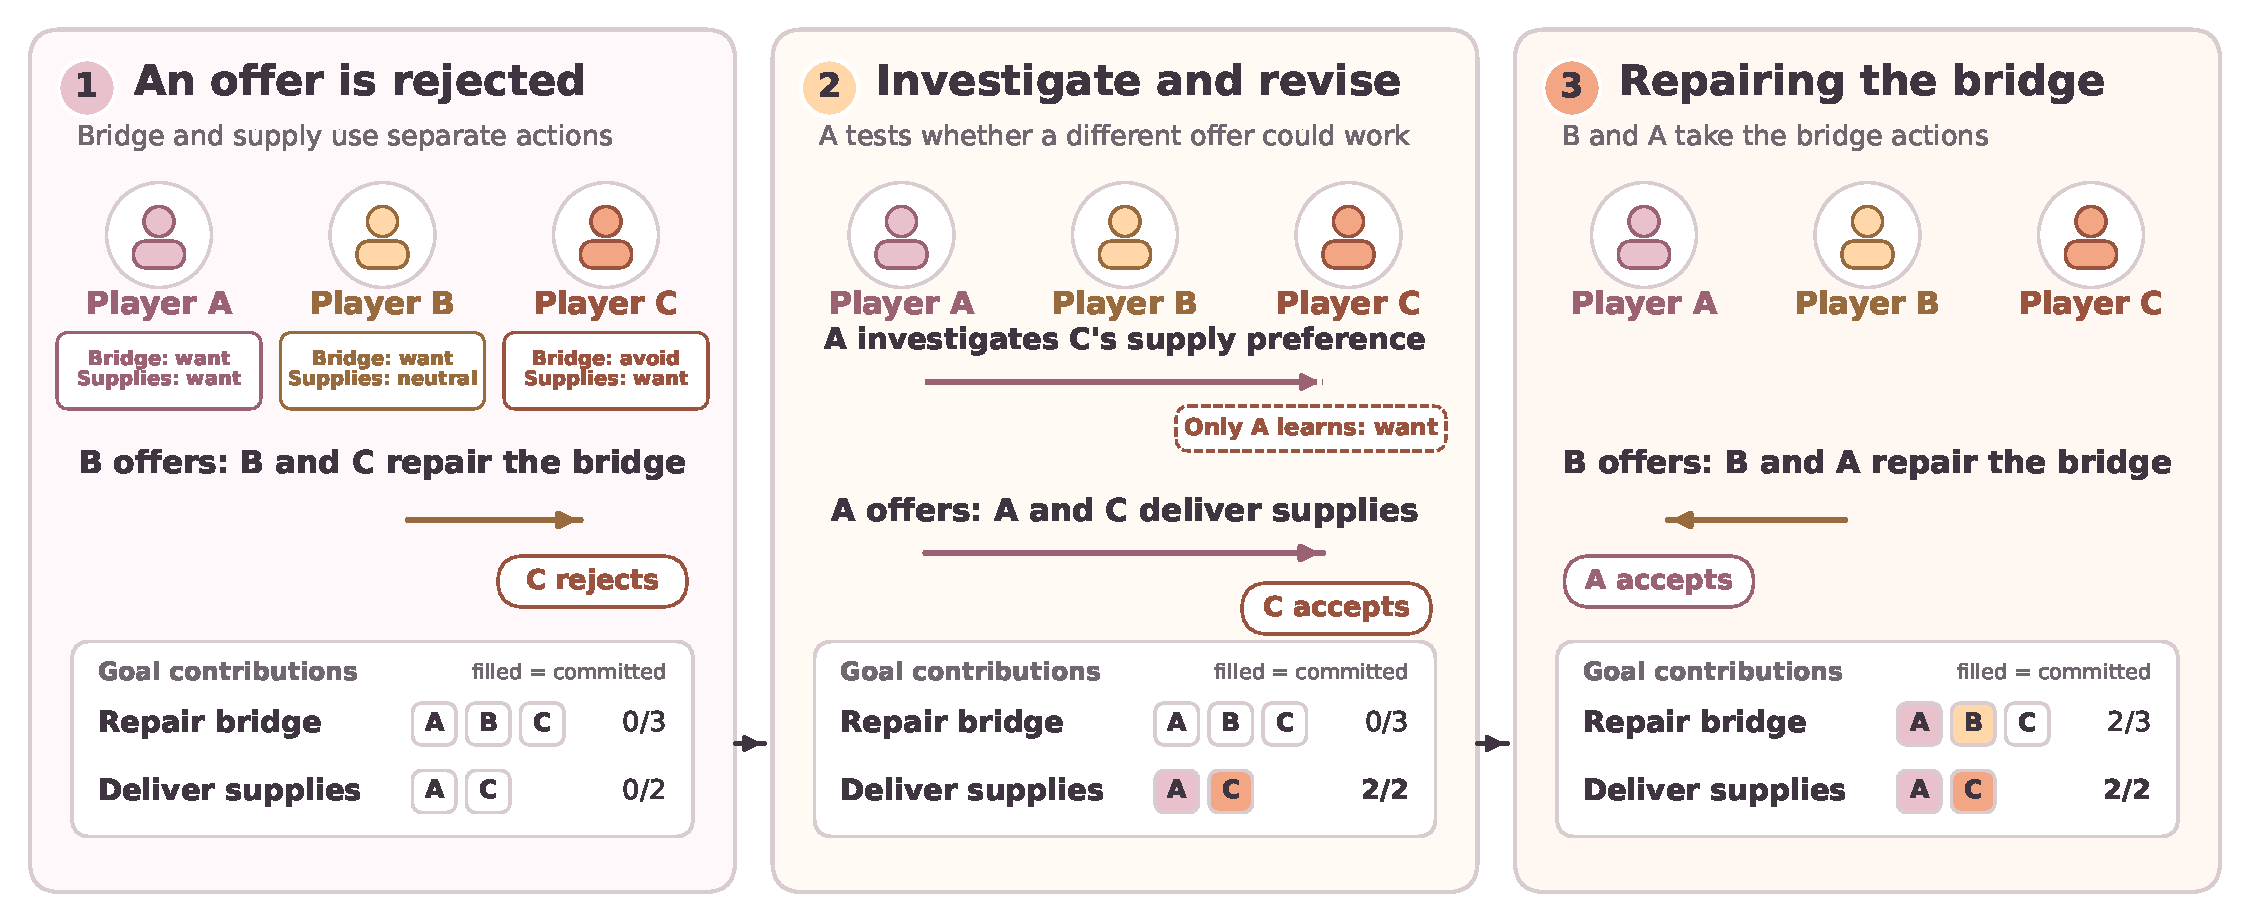
\includegraphics[width=\textwidth]{figures/game_flow.pdf}
\caption{An illustrative three-player negotiation with private preferences
and two linearly scored goals. \emph{Repair bridge} requires distinct bridge
actions from A, B, and C; \emph{Deliver supplies} requires distinct supply
actions from A and C. A filled letter indicates that player's commitment to
that particular goal, and the fractions show goal progress. B first offers
bridge actions to C, who rejects: accepting would leave the bridge at $2/3$
and give C $-2/3$ from a goal it dislikes if play stopped then. A investigates
C's supply preference and privately learns that C wants supplies. After C
passes, B investigates A's bridge preference and privately learns that A
wants the bridge. A then offers to deliver supplies with C, who accepts,
completing that goal. C passes again before B offers bridge actions to A,
who accepts, bringing bridge progress to $2/3$; C does not join it. The
game ends after this final offer. Proposer turns follow the fixed round-robin
order B--A--C throughout. This adapted legal sequence
illustrates the rules and hidden preferences, without asserting optimal
play.}
\label{fig:game-flow}
\end{figure}

\subsection{Game Slices and Oracle Solver}
\label{sec:game-slices}

A \emph{game slice} is a consecutive segment of play that begins at a chosen
decision and may include later decisions. For example, it can contain an
offer, the partner's response, and the next proposal. The slice records which
actions occurred and what each player observed following the game rule.
At decision $s$, the acting player $i$
knows the public history $h_s$, its own preferences $v_i$, and its private
answers $r_s^i$. We write this view as $I_s^i=(h_s,v_i,r_s^i)$, an
\emph{information set} that identifies the game states the player cannot
distinguish~\citep{kuhn1953extensive}. The observed sequence locates the
decisions to be labeled. For each such decision, the oracle also evaluates
actions that were not taken and their possible continuations; it does not
give the acting player access to the partners' hidden preferences. A formal
slice definition appears in Appendix~\ref{app:oracle}. Following the Bayesian
representation of private types
\citep{harsanyi1967games}, the oracle solves the finite tree over possible
preferences and actions under the common prior $\mu_0$.
A \emph{policy} $\pi_i(a\mid I)$ assigns a probability to each legal action
$a\in\mathcal L(I)$ given what player $i$ can know. Let $\Pi_i$ contain all
such policies, including plans for later decisions after each possible
observation; $\pi_{-i}$ denotes the other players' policies. Holding
$\pi_{-i}$ fixed, a \emph{best response} maximizes player $i$'s expected
terminal utility over these complete plans. Starting from uniform legal
actions, we update every player against the same previous policy profile:
\begin{align}
 \operatorname{BR}_i(\pi_{-i})
 &\in\arg\max_{\widetilde\pi_i\in\Pi_i}
 \mathbb E_{\mu_0,(\widetilde\pi_i,\pi_{-i})}
 [U_i(C_T;v_i)],\nonumber\\
 \pi_i^{(0)}(a\mid I)&=|\mathcal L(I)|^{-1},\qquad
 \pi_i^{(k+1)}=\operatorname{BR}_i(\pi_{-i}^{(k)}).
 \label{eq:oracle-iteration}
\end{align}
We retain a fixed profile $\pi^\star$ only if it passes a
no-profitable-unilateral-deviation check, following the stability criterion
of \citet{nash1950equilibrium}: in every initial private-information class,
no player can improve its expected utility by changing its complete plan
while the others keep theirs. At
\textsc{accept}/\textsc{reject} responses, expected utility to the other
players breaks ties in the responder's own utility; remaining ties are mixed
uniformly. The reference policy also turns interaction into an inference target. Let
$b_s^{i,\star}(v_{-i})=\Pr_{\mu_0,\pi^\star}(v_{-i}\mid I_s^i)$ be player $i$'s
\emph{posterior}, its probability distribution over the others' hidden
preferences. If partner $j$ autonomously chooses $a_s^j$, Bayes' rule gives
\begin{equation}
 b_{s+1}^{i,\star}(v_{-i})\ \propto\
 b_s^{i,\star}(v_{-i})
 \pi_j^\star(a_s^j\mid I_s^j(v_i,v_{-i})),\qquad j\ne i.
 \label{eq:oracle-update-main}
\end{equation}
An action is evidence to the extent that the reference policy makes it more
likely under one candidate preference assignment than another. For planning,
we instead ask what would happen if $i$ chose each legal action $a$ now:
\begin{equation}
 Q_i^\star(I_s^i,a)=
 \mathbb E_{\mu_0,\pi^\star}
 [U_i(C_T;v_i)\mid I_s^i,\operatorname{do}(a_s^i=a)].
 \label{eq:oracle-targets}
\end{equation}
The forced action is followed by the reference policy for the rest of the
game. Across a longer slice, each player's posterior is updated from the
observations available to that player and informs its later decisions.
Appendix~\ref{app:oracle} details the computation and validity checks;
Section~\ref{sec:experiment-training} describes slice construction and sampling.
